\section{Operational law}

Operational laws serve as straightforward equations that offer an abstract representation or model of the average behavior of various systems. 
These laws are highly general and impose minimal assumptions about the behavior of the random variables characterizing the system.
One notable advantage of these laws lies in their simplicity; they can be swiftly and easily applied. 
They are based on observable variables, which are values that we could derive from observing a system over a finite period.
The underlying assumptions include:
\begin{itemize}
    \item The system receives requests from its environment.
    \item Each request generates a job or customer within the system.
    \item Upon processing the job, the system responds to the environment by completing the corresponding request.
\end{itemize}

\paragraph*{Measurable variables}
When observing such an abstract system, we might measure the following quantities:
\begin{itemize}
    \item $T$: the length of time we observe the system.
    \item $A$: the number of request arrivals we observe.
    \item $C$: the number of request completions we observe.
    \item $B$: the total amount of time during which the system is busy, where $B \leq T$.
    \item $N$: the average number of jobs in the system.
\end{itemize}
\begin{figure}[H]
    \centering
    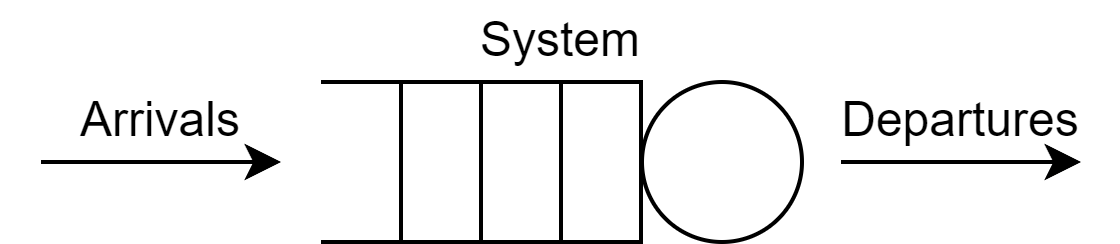
\includegraphics[width=0.5\linewidth]{images/qn.png}
    \caption{Queueing network}
\end{figure}
From these observed values, we can derive the following four important quantities:
\begin{itemize}
    \item $\lambda=\frac{A}{T}$: the arrival rate. 
    \item $X=\frac{C}{T}$: the throughput or completion rate.
    \item $U=\frac{B}{T}$: the utilization.
    \item $S=\frac{B}{C}$: the mean service time per completed job.
\end{itemize}
We will assume that the system is job flow balanced, meaning that the number of arrivals is equal to the number of completions during an observation period, i.e., $A=C$. 
This assumption is testable because an analyst can verify whether it holds true. 
It can be strictly satisfied by selecting a suitable measurement interval.
Note that if the system is job flow balanced, the arrival rate will be the same as the completion rate, that is:
\[\lambda=X\]

\paragraph*{Operational law}
A system can be viewed as comprising several devices or resources, each of which can be treated as a system on its own within the framework of operational laws.
Each of these devices or resources can be considered a system in its own right within the framework of operational laws.
An external request triggers a job within the system, which may then circulate among the resources until all necessary processing is completed. 
As it reaches each resource, it is treated as a request, generating a job internal to that resource.
A system can thus be seen as comprising multiple devices or resources, each of which can be analyzed individually as a system under operational laws.
We define the following variables:
\begin{itemize}
    \item $T$: the length of time we observe the system.
    \item $A_k$: the number of request arrivals we observe for resource $k$. 
    \item $C_k$: the number of request completions we observe at resource $k$. 
    \item $B_k$: the total amount of time during which resource $k$ is busy ($B_k\leq T$). 
    \item $N_k$: the average number of jobs in resource $k$  (either in queue or being served).
\end{itemize}
From these observed values, we can derive the following four important quantities for resource $k$:
\begin{itemize}
    \item $\lambda_k=\frac{A_k}{T}$: the arrival rate. 
    \item $X_k=\frac{C_k}{T}$: the throughput or completion rate.
    \item $U_k=\frac{B_k}{T}$: the utilization.
    \item $S_k=\frac{B_k}{C_k}$: the mean service time per completed job.
\end{itemize}

\subsection{Utilization law}
Using the previously determined observed values, we find:
\[X_k S_k = \dfrac{C_k}{T} \cdot \dfrac{B_k}{C_k} = \dfrac{B_k}{T}=U_k\]
From this, we derive the utilization law as:
\[U_k=X_k S_k\]

\subsection{Little's law}
Little's Law states:
\[N = XR\]
Here, $N$ is the average number of requests in the system, $X$ is the system throughput, measured in requests per second, and $R$ is the average system residence time per request.
Little's Law can be applied to the entire system as well as to some subsystems.
If the system throughput is $X$ requests per second, and each request remains in the system on average for $R$ seconds, then for each unit of time, we can observe on average $XR$ requests in the system.

\paragraph*{Little's law derivation}
Let's denote $W$ as the accumulated time in the system (in jobs-seconds).
Then, we can express:
\begin{itemize}
    \item $N$, the average number of requests in the system, as $N=\frac{W}{T}$.
    \item $R$, the average system residence time per request, as $R=\frac{W}{C}$.
\end{itemize}
Thus, we can write:
\[N=\dfrac{W}{T}=\dfrac{C}{T}\cdot\dfrac{W}{C}=XR\]
Thus, $N = XR$. 

\paragraph*{Little's law level 1}
Little's Law can be applied to the single server disk (without the queue).
In this case:
\begin{itemize}
    \item $N(1)$ represents the percentage of time in which the disk server is busy, corresponding to $U_{\text{disk}}$. 
    \item $R(1)$ represents the average service time of requests.
    \item $X(1)$ represents the rate of serving requests.
\end{itemize}

\paragraph*{Little's Law level 2}
Now, let's include the queue.
In this context:
\begin{itemize}
    \item $N(2)$ represents the number of users in the service center (waiting and in service).
    \item $R(2)$ is the time spent in the service center (waiting time and service time).
    \item $X(2)$ is the throughput of the disk server and corresponds to $X(1)$.
\end{itemize}

\paragraph*{Little's Law level 3}
Let's focus on the central subsystem.
In this scenario:
\begin{itemize}
    \item $N(3)$ represents the total number of users in the subsystem (e.g., requests for web pages per second).
    \item $R(3)$ represents the average time spent in the subsystem by each request.
    \item $X(3)$ is the subsystem throughput (e.g., number of web pages served per second).
\end{itemize}

\paragraph*{Little's Law level 4}
Now, let's consider the complete system.
Here:
\begin{itemize}
    \item $N(4)$ is the total number of users in the system, which is fixed since we have a closed system.
    \item $R(4)$ is the total amount of time spent in service, waiting, and at the client-side terminals (think time, e.g., the time a user spends reading a web page and processing a request).
    \item $X(4)$ is the rate at which requests reach the system from the client terminals, corresponding to $X(3)$. 
\end{itemize}

\subsection{Interactive response time law}
Back when most processing was done on shared mainframes, think time $Z$ was quite literally the length of time that a programmer spent thinking before submitting another job.
More generally, in interactive systems, jobs spend time in the system not engaged in processing or waiting for processing. 
This may be because of interaction with a human user or for some other reason. 
The think time represents the time between processing being completed and the job becoming available as a request again.

The interactive response time law states:
\[R =\dfrac{N}{X}-Z\]
The response time in an interactive system is the residence time minus the think time.
Note that if the think time is zero ($Z=0$), then $R =\frac{N}{X}$, and the interactive response time law simplifies to Little's Law.

\subsection{Forced Flow Law}
During an observation interval, we can tally not only completions external to the system but also the number of completions at each resource within the system.

Let $C_k$ be the number of completions at resource $k$. 
We define the visit count, $V_k$ of the $k$-th resource to be the ratio of the number of completions at that resource to the number of system completions:
\[V_k=\dfrac{C_k}{C}\]
It's important to note that:
\begin{itemize}
    \item If $C_k>C$, resource $k$ is visited several times on average during each system-level request. 
        This occurs when there are loops in the model.
    \item If $C_k<C$, resource $k$ might not be visited during each system-level request.
        This can happen if there are alternatives (e.g., caching of disks).
    \item If $C_k=C$, resource $k$ is visited on average exactly once every request.
\end{itemize}
The forced flow law captures the relationship between the different components within a system. 
It states that the throughput or flows in all parts of a system must be proportional to one another.
\[X_k=V_kX\]
The throughput at the $k$-th resource is equal to the product of the throughput of the system and the visit count at that resource.
By rewriting $C_k=V_kC$ and applying $\frac{C_k}{T}=V_k\frac{C}{T}$, we can derive the forced flow law:
\[X_k=V_kX\]

\subsection{Utilization Law with visits}
If we are aware of the processing required by each job at a resource, we can calculate the resource's utilization.
Let's assume that each time a job visits the $k$-th resource, it requires a certain amount of processing, denoted by $S_k$.
It's important to note that the service time $S_k$ is not necessarily the same as the response time of the job at that resource. 
Generally, a job might have to wait for some time before processing begins.

The total amount of service that a job in the system generates at the $k$-th resource is termed the service demand, denoted as $D_k$: 
\[D_k=S_kV_k\]
The utilization of a resource, represented by $U_k$, indicates the percentage of time the $k$-th resource is in use processing a job.
As a result, the utilization law can be expressed as:
\[U_k=X_kS_k=(XV_k)S_k=D_kX\]
The utilization of a resource is equal to the product oft the throughput of that resource and the average service time at that resource, and the system-level throughput and the average service demand at that resource: 
\[U_k=D_kX\]

The average service time $S_k$ accounts for the average time a job spends at station $k$ when it is served.
The average service demand $D_k$ accounts for the average time a job spends at station $k$ during its stay in the system. 
Depending on how jobs move in the system, the demand can be less than, greater than, or equal to the average service time of station $k$. 

\subsection{Response and residence times}
When considering nodes characterized by visits different from one, we can define two permanence times:
\begin{itemize}
    \item \textit{Response time $\tilde{R}_k$}: this accounts for the average time spent in station $k$ when the job enters the corresponding node. 
        It represents the time for the single interaction, such as a disk request.
    \item \textit{Residence time $R_k$}: this accounts for the average time spent by a job at station $k$ during its stay in the system. 
        It can be greater or smaller than the response time depending on the number of visits.
\end{itemize}
It's important to note the relation between residence time and response time is similar to the one between demand and service time:
\[\begin{cases}
    D_k=V_kS_k \\
    R_k=V_k\tilde{R}_k
\end{cases}\]
Also, note that for single queue open systems or tandem models, $V_k=1$. 
This implies that the average service time and service demand are equal, and response time and residence time are identical.

\subsection{General response time law}
One method of computing the mean response time per job in a system is to apply Little's Law to the system as a whole. 
However, if the mean number of jobs in the system, $N$, or the system-level throughput, $X$, are not known, an alternative method can be used.

Applying Little's Law to the $k$-th resource, we find that: 
\[N_k=X_k\tilde{R}_k\]
Here, $N_k$ is the mean number of jobs at the resource, and $\tilde{R}_k$ is the average time spent at the resource for a single interaction (e.g., a disk request).

From the forced flow law, we know that $X_k=XV_k$. 
Thus, we can deduce that:
\[\dfrac{N_k}{X}=V_k\tilde{R}_k=R_k\]
The total number of jobs in the system is clearly the sum of the number of jobs at each resource, i.e. $N = N_1 +\cdots+ N_M$ if there are $M$ resources.

From Little's Law $R=\frac{N}{X}$, and so, $R_k=\frac{N_k}{X}=V_k\tilde{R}_k$: 
Thus, the general response time law is:
\[R=\sum_kV_k\tilde{R}_k=\sum_kR_k\]

The average response time of a job in the system is the sum of the product of the average time for the individual access at each resource and the number of visits it makes to that resource. 
The average response time of a job in the system is the sum of the resources' residence time.

\subsection{Summary}
Operational laws offer simple equations that serve as an abstract representation or model of the average behavior of nearly any system. 
These laws are highly general and make minimal assumptions about the behavior of the random variables characterizing the system.
Moreover, their simplicity allows for quick and easy application, making them valuable tools in system analysis and modeling.